\documentclass[12pt]{report}
\usepackage[print,nopanel]{pdfscreen}
%\begin{print}
\usepackage{lipsum}% http://ctan.org/pkg/lipsum
\usepackage{titletoc}% http://ctan.org/pkg/titletoc
%\section{type}
\usepackage{lastpage}
\usepackage{macro/macro}
\usepackage{float}
\usepackage{wrapfig}
\usepackage{fancyhdr}
\usepackage{verbatim}
%Options: Sonny, Lenny, Glenn, Conny, Rejne, Bjarne, Bjornstrup
\usepackage[Glenn]{fncychap}
\lhead{\large\bfseries CAD Development}
\usepackage[left=2.5cm, right=1.5cm, top=2.5cm, bottom=1.5cm]{geometry}
\pagestyle{fancy}
%\end{print}
\margins{.5cm}{.5cm}{.5cm}{.5cm}
\begin{screen}

\renewcommand{\encodingdefault}{T1}
\usepackage{setspace}
\linespread{1.5}
\renewcommand{\rmdefault}{ptm}
\end{screen}
\screensize{8cm}{9cm}
\overlay{overlay8.pdf}
\usepackage{graphicx}

\begin{document}
\newcommand{\centertext}[1]{\begin{center}\textbf{#1}\end{center}}
\newcommand{\student}{\vskip 2.5cm}
\newcommand{\supervisor}{\vskip 2cm}
\newcommand{\stamp}{\vskip 2.5cm}
\newcommand{\HRule}{\rule{\linewidth}{0.5mm}}
\newcommand{\projecttitle}{\Huge \bf{CAD Development}\vskip 0.5in}
\newcommand{\tab}[1]{\hspace{.4\textwidth}\rlap{#1}}
\newcommand{\itab}[1]{\hspace{.05\textwidth}\rlap{#1}}
\newcommand{\logo}[1]{\includegraphics[scale=0.7]{#1}}
\newcommand{\submitted}{
\vskip 0.4in
\textnormal{Submitted for partial fulfilment of the Degree\\
of\\
Bachelor of Technology\\
(Computer Science and Engineering)\\
}
\vskip 2.5cm
%\image{0.7}{images/gne.jpg}{}
\logo{images/gne.jpg}
\vskip 3.0cm
\begin{minipage}{0.4\textwidth}
\begin{flushleft} \large
{Submitted By:}\\
\textnormal{Gurpinder Singh\\
1243630\\ 125026} % Your name
\end{flushleft}
\end{minipage}
~
\begin{minipage}{0.4\textwidth}
\begin{flushright} \large
{Submitted To:} \\
\textnormal{Sukhjit Singh Sehra\\
Training Coordinator\\                                                                                                                          
CSE Department} % Supervisor's Name
\end{flushright}
\end{minipage}\\[2cm]
\HRule \\[0.4cm]

\textnormal{Department of Computer Science \& Engineering \\
Guru Nanak Dev Engineering College \\
Ludhiana 141006}
}


\newcommand{\pagetitle}{\begin{center}
\projecttitle
\Large\textbf{}\\
\submitted
\vskip 1cm

\end{center}}
\newcommand{\openoffice}{\textbf{OpenOffice}}
\newcommand{\frontmatter}[1]{\begin{Large} \textbf{#1} \end{Large}}
\newcommand{\ppttitle}{\begin{center}
\end{center}}


\begin{screen}
\ppttitle
\end{screen}
\footskip 0.7cm
\thispagestyle{empty} 
\pagetitle
\newpage
\pagenumbering{Roman}
\cfoot{\thepage}

\begin{Large}
\centertext{Acknowledgement}
\end{Large}
I, student of Guru Nanak Dev Engineering College, Ludhiana, have taken efforts in this project.
However, it would not have been possible without the kind support and help of many individuals
and organizations. I would like to extend my sincere thanks to all of them.\\
The author is highly grateful to Dr. M.S. Saini Director, Guru Nanak Dev Engineering College, Ludhiana for providing him with the opportunity to carry out his Six Weeks Training at
Testing and Consultancy Cell, Guru Nanak Dev Engineering College, Ludhiana.\\
The author would like to whole heartedly thank Dr. H.S. Rai Dean, Testing and Consultancy
Cell, Guru Nanak Dev Engineering College, Ludhiana who is a vast sea of knowledge and without whose constant and never ending support and motivation, it would never have been possible to complete the project and other assignments so efficiently and effectively.\\
Finally, the authors are indebted to all whosoever have contributed in
this report work with Mandeep Singh (D3 CSE) and all other trainees. Without their 
encouragement, it would not have been possible to complete this project
in such an efficient manner.





\vskip 1.0cm 
\noindent Gurpinder Singh

\newpage

\begin{Large}
\centertext{Abstract}
\end{Large}

\noindent CAD development project discuss the work done in computer-aided-design. Computer-aided design (CAD) is the use of computer systems to assist in the creation, modification, analysis, or optimization of a design. I explored  LibreCAD  Source  Code. LibreCAD is Free and Open Source CAD Software. LibreCAD is a  fully  comprehensive  2D  CAD   application  that  you  can  download  and  install  for  free.  There  is  a  large base  of  satisfied  LibreCAD   users  worldwide,  and  it  is  available  in  more  than  20  languages  and  for  all
major  operating  systems,  including  Microsoft  Windows,  Mac  OS  X  and  Linux .  Librecad  is  an  application  for  computer  aided  design  in  two dimensions  .  With  librecad   you   can  create  technical  drawings  such  as  plans  for  buildings,  interiors,
mechanical parts or schematics and diagrams. Basically, LibreCAD is used to make 2D design. \\
\noindent This project also includes work regarding qt creater to make a text editor. Qt Creator is a cross-platform C++, JavaScript and QML integrated development environment which is part of the SDK for the Qt GUI Application development framework.\\ 
\noindent Furthermore, this project involves hatching technique implementation using C++ and Cairo graphics library. Hatching is the technique to fill any closed contour with different patterns or colors and is used by many CAD softwares.\\
\noindent Also, this project is completely open source and the entire code is available 
to the user as and when required. There is also Complete developer's 
Documentation as well as User manual alongwith it that helps using it a lot easier.

\newpage
\tableofcontents
\newpage
\listoffigures
\newpage

\pagenumbering{arabic}
\cfoot{\thepage}

\newpage
\chapter{Introduction To Organisation}
\begin{figure}[ht]
\centering
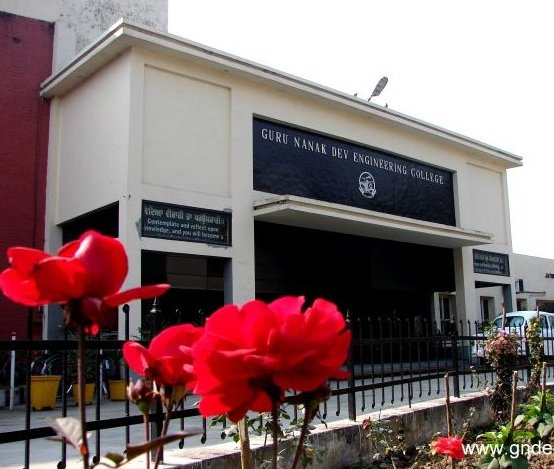
\includegraphics[scale=0.5]{images/gndec.jpg}
\caption{Guru Nanak Dev Engineering College}
\end{figure}
\hspace{-1.7em} I had my Six Weeks Industrial Training at TCC-Testing And Consultancy Cell, GNDEC Ludhiana. Guru Nanak Dev Engineering College was established by the Nankana
Sahib Education Trust Ludhiana. The Nankana Sahib Education Trust i.e NSET
was founded in memory of the most sacred temple of Sri Nankana Sahib, birth place
of Sri Guru Nanak Dev Ji. With the mission of Removal of Economic Backwardness
through Technology Shiromani Gurudwara Parbandhak Committee i.e SGPC started a
Poly technical was started in 1953 and Guru Nanak Dev Engineering College was established in 1956.\\\\
NSET resolved to uplift Rural areas by admitting 70\% 
of students from these rural
areas ever year. This commitment was made to nation on 8th April, 1956, the day
foundation stone of the college building was laid by Dr. Rajendra Prasad Ji, the First
President of India. The College is now ISO 9001:2000 certified.\\\\
Guru Nanak Dev Engineering College campus is spread over 88 acres of prime land
about 5 Km s from Bus Stand and 8 Km s from Ludhiana Railway Station on Ludhiana-Malerkotla Road. The college campus is well planned with beautifully laid out tree plantation, pathways, flowerbeds besides the well maintained sprawling lawns all around. It
has beautiful building for College,Hostels,Swimming Pool,Sports and Gymnasium Hall
Complex, Gurudwara Sahib, Bank, Dispensary, Post Office etc. There are two hostels
for boys and one for girls with total accommodation of about 550 students. The main
goal of this institute is:\\\\
\begin{itemize}
\item To build and promote teams of experts in the upcoming specialisations.
\item To promote quality research and undertake research projects keeping in view their
relevance to needs and requirements of technology in local industry.
\item To achieve total financial independence.
\item To start online transfer of knowledge in appropriate technology by means of establishing multipurpose resource centres.
\end{itemize}
\section{Testing and Consutancy Cell}
My Six Weeks Institutional Training was done by me at TCC i.e Testing And
Consultancy Cell,
GNDEC Ludhiana under the guidance of Dr. H.S.Rai Dean Testing and Consultancy Cell.
Testing and Consultancy Cell was established in the year 1979 with a basic aim to produce
quality service for technical problems at reasonable and affordable rates as a service to society
in general and Engineering fraternity in particular.\\
\begin{figure}[ht]
\centering
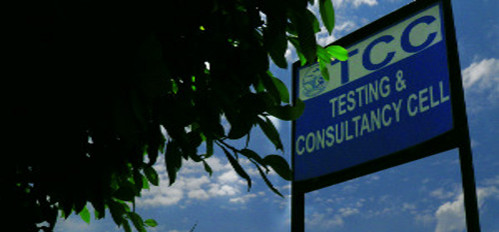
\includegraphics[scale=0.7]{images/aw.jpg}
\caption{Testing and Consultancy Cell}
\end{figure}
\hspace{-1.7em} Consultancy Services are being rendered by various Departments of the College to the
industry, Sate Government Departments and Entrepreneurs and are extended in the form of
expert advice in design, testing of materials \& equipment, technical surveys, technical audit,
calibration of instruments, preparation of technical feasibility reports etc.
This consultancy cell of the college has given a new dimension to the development
programmers of the College. Consultancy projects of over Rs. one crore are completed by the
Consultancy cell during financial year 2009-10. \\ \\
Ours is a pioneer institute providing Consultancy Services in the States of Punjab, Haryana,
Himachal, J\&K and Rajasthan. Various Major Clients of the Consultancy Cell are as under:\\
\begin{itemize}
\item Northern Railway, Govt. of India
\item Indian Oil Corporation Ltd.
\item Larson \& Turbo.
\item Multi National Companies like AFCON \& PAULINGS.
\item Punjab Water Supply \& Sewage Board
\item Power Grid Corporation of India.
\item National Building Construction Co.
\item Punjab State Electricity Board.
\item Punjab Mandi Board.
\item Punjab Police Housing Corporation.
\item National Fertilizers Ltd.
\item GLADA, Ludhiana
\end{itemize}


\newpage
%\chapter{\LaTeX}
%\section{Introduction to \LaTeX}

\LaTeX, I had never heard about this term before doing this project,
but when I came to know about its features, found it excellent. 
\LaTeX{} (pronounced /ˈleɪtɛk/, /ˈleɪtɛx/, /ˈlɑːtɛx/, or /ˈlɑːtɛk/) is a 
document markup language and document preparation system for the \TeX{} 
typesetting  program. Within the typesetting system, its name is styled 
as \LaTeX.

\image{0.9}{images/donald.png}{Donald Knuth, Inventor Of \TeX{} 
typesetting system}

Within the typesetting system, its name is styled as \LaTeX. The term 
\LaTeX{} refers only to the language in which documents are written, 
not to the editor used to write those documents. In order to create a 
document in \LaTeX, a .tex file must be created using some form of text 
editor. While most text editors can be used to create a \LaTeX{} document, 
a number of editors have been created specifically for working with \LaTeX.

\LaTeX{} is most widely used by mathematicians, scientists, 
engineers, philosophers, linguists, economists and other scholars in 
academia. As a primary or intermediate format, e.g., translating DocBook 
and other XML-based formats to PDF, \LaTeX{} is used because of the 
high quality of typesetting achievable by \TeX. The typesetting system 
offers programmable desktop publishing features and extensive facilities 
for automating most aspects of typesetting and desktop publishing, 
including numbering and cross-referencing, tables and figures, 
page layout and bibliographies.

\LaTeX{} is intended to provide a high-level language that
accesses the power of \TeX. \LaTeX{} essentially comprises a
collection of \TeX{} macros and a program to process \LaTeX documents. 
Because the \TeX{} formatting commands are very low-level, it is usually 
much simpler for end-users to use \LaTeX{}.


\subsection{Typesetting}
\LaTeX{} is based on the idea that authors should be able to focus on 
the content of what they are writing without being distracted by its 
visual presentation. In preparing a \LaTeX{} document, the author 
specifies the logical structure using familiar concepts such as 
chapter, section, table, figure, etc., and lets the \LaTeX{} system 
worry about the presentation of these structures. It therefore 
encourages the separation of layout from content while still allowing 
manual typesetting adjustments where needed. 

\begin{verbatim}
\documentclass[12pt]{article}
\usepackage{amsmath}
\title{\LaTeX}
\date{}
\begin{document}
  \maketitle 
  \LaTeX{} is a document preparation system 
  for the \TeX{} typesetting program.
   \par 
   $E=mc^2$
\end{document}
\end{verbatim}
\image{0.3}{images/latexoutput.png}{\LaTeX{} output of above program.}

\subsection{Installing \LaTeX{} on System}
Installation of \LaTeX{} on personal system is quite easy. As i have used \LaTeX{} on Ubuntu 13.04 so i am discussing the installation steps for Ubuntu 13.04 here:
\begin{itemize}
\item Go to terminal and type\\\\
\textit{sudo apt-get install texlive-full}
\item Your Latex will be installed on your system and you can check for manual page by typing.\\\\
\textit{man latex}\\
in terminal which gives manual for latex command.\\
\item To do very next step now one should stick this to mind that the document which one is going to produce is written in any type of editor whether it may be your most common usable editor Gedit or you can use vim by installing first vim into your system using command.\\\\
\textit{sudo apt-get install vim}\\
\item After you have written your document it is to be embedded with some set of commands that Latex uses so as to give a structure to your document. Note that whenever you wish your document to be looked into some other style just change these set of commands.\\\\
\item When you have done all these things save your piece of code with .tex format say test.tex. Go to terminal and type\\\\
\textit{latex path of the file test.tex Or pdflatex path of the file test.tex\\ eg: pdflatex test.tex}\\
for producing pdf file simultaneously.\\
After compiling it type command\\\\
\textit{evince filename.pdf\\ eg: evince test.pdf}\\
To see output pdf file. 
\end{itemize}

\subsection{Graphical Editors for \LaTeX{}}
\LaTeX{} is not restricted to command line only there are so many graphical based editors available to be used. These GUi based editors provide an easy interface to user so as to do typesetting in an efficient manner. Some of them are listed below:
\begin{itemize}
\item {Texmaker}
\begin{figure}[ht]
\centering
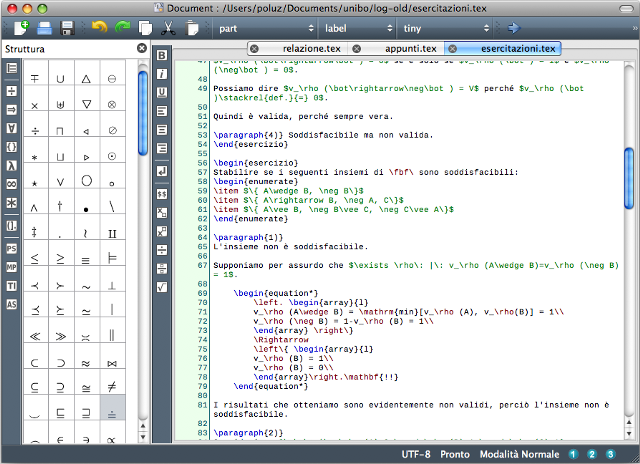
\includegraphics[scale=0.4]{images/texmaker.png}
\caption{Texmaker, A Graphical \LaTeX{} Editor}
\end{figure}
\item LEd
\begin{figure}[ht]
\centering
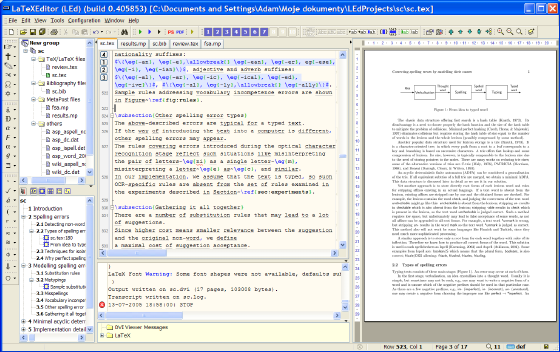
\includegraphics[scale=0.5]{images/led.png}
\caption{LEd, A Graphical \LaTeX{} Editor}
\end{figure}
\end{itemize}
And many more but the preferred method to produce \LaTeX{} document is through console mode only.


\subsection{Pdfscreen \LaTeX{}}
There are some packages that can help to have unified document using \LaTeX{}. Example of such a package is pdfscreen that let the user view it’s document in two forms-print and screen. Print for hard copy and screen for viewing your document on screen. Download this package from www.ctan.org/tex-archive/macros/latex/contrib/pdfscreen/.\\
Then install it using above mention method.\\
To test it the test code is given below:-\\
Just changing print to screen gives an entirely different view. But for working of pdfscreen another package required are comment and fancybox.\\\\
The fancybox package provides several different styles of boxes for framing and rotating content in your document. Fancybox provides commands that produce square-cornered boxes with single or double lines, boxes with shadows, and round-cornered boxes with normal or bold lines. You can box mathematics, floats, center, flushleft, and flushright, lists, and pages.\\\\
Whereas comments package selectively include/excludes portions of text. The comment package allows you to declare areas of a document to be included or excluded. One need to make these declarations in the preamble of your file. The package uses a method for exclusion that is pretty robust, and can cope with ill-formed bunches of text.\\\\
So these extra packages needed to be installed on system for the proper working of pdfscreen package.
\subsection{Web based graphic generation using \LaTeX{}}
\LaTeX{} is also useful when there is need of generating the graphics from browser. For
example to draw a circle by just entering its radius in html input box. So this kind
A
of project can be conveniently handled using \LaTeX{}. Basic idea behind this generation
process is that when user clicks on submit button after entering radius a script will run
that enter the radius in already made .tex file and recompiles it on server and makes its
pdf and postscript file. After that user can view those files by clicking on link provided
to view the files. See some screen shots of such a graphic generation project made by
Dr. H.S. Rai:\\
So here in the above input page which is also the index page user can enter input
for length of rectangle, breadth of rectangle and for radius of circle after that user can submit the values. After the values get submitted a script get runs by php code at server
side. This script first enters the dimensions of rectangle and circle that were selected by
user in to an already existing .tex file and replace with the older dimensions there. After
that script recompiles the the tex file and make it available for user.\\
In above figure it gets clear that .tex file has been compiled and pdf and postscript files
are available to user and user can download the graphics so produced. Hence graphics
can be generated in \LaTeX{} through web interface.
\begin{figure}[ht]
\centering
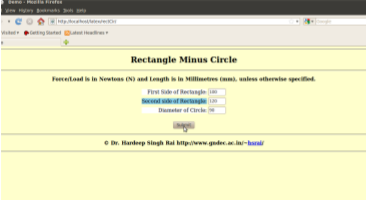
\includegraphics[scale=0.5]{images/webgraphic.png}
\caption{Web based graphic generation using \LaTeX{}(input page)}
\end{figure}

\chapter{Introduction To Project}
\section{Introduction}
The  term  computer  graphics  includes  almost  everything  on  computers  that  is  not  text  or  sound.  Today
almost  every  computer  can  do  some  graphics,  and  people  have  even  come  to  expect  to  control  their
computer  through  icons  and  pictures  rather  than  just  by  typing.  Here  in  our  lab  at  the  Program  of
Computer  Graphics,  we  think  of  computer  graphics  as  drawing  pictures  on  computers,  also  called
rendering.  The  pictures  can  be photographs, drawings, movies, or simulations ­­ pictures of things which
do  not  yet  exist  and  maybe  could   never  exist.  Or  they  may  be  pictures  from  places  we  cannot  see
directly,  such  as  medical  images  from  inside  your  body.  Computer  graphics  is  now  used  in  various
fields;  for  industrial,  educational,  medical  and  entertainment  purposes.  The  aim  of  computer  graphics  is
to  visualize  real  objects  and  imaginary  or  other  abstract  items.  In  order to visualize various things, many
technologies  are  necessary  and  they  are  mainly  divided  into  two  types  in  computer  graphics:  modeling
and  rendering  technologies.\\

\section{Introduction to CAD}
Computer-aided design (CAD) is the use of computer systems to assist in the creation, modification, analysis, or optimization of a design. CAD software is used to increase the productivity of the designer, improve the quality of design, improve communications through documentation, and to create a database for manufacturing.CAD is an important industrial art extensively used in many applications, including automotive, shipbuilding, and aerospace industries, industrial and architectural design, prosthetics, and many more. CAD is also widely used to produce computer animation for special effects in movies, advertising and technical manuals. CAD output is often in the form of electronic files for print, machining, or other manufacturing operations. CAD is also used for the accurate creation of photo simulations that are often required in the preparation of Environmental Impact Reports, in which computer-aided designs of intended buildings are superimposed into photographs of existing environments to represent what that locale will be like were the proposed facilities allowed to be built.  Computer­ Aided  Drafting  describes  the  process  of  creating  a
technical  drawings with the use of computer software. CAD software is used to increase the productivity
of  the  designer,  improve  the  quality  of  design,  improve  communications  through  documentation,  and  to
create  a  database  for  manufacturing.  CAD  output  is  often  in  the  form  of  electronic  files  for  print  or
machining  operations.  CAD  software  uses  either  vector  based  graphics  to  depict  the  objects  of
traditional  drafting,  or  may  also  produce  raster  graphics  showing  the  overall   appearance  of  designed
objects.\\
  Today  there  are  very  few  aspects  of  our  lives  not  affected  by  computers.  Practically  every  cash or
monetary  transaction  that  takes  place  daily  involves  a  computer.  In  many  cases,  the  same  is  true  of
computer  graphics.  Whether  you  see  them  on  television,  in  newspapers,  in  weather   reports  or  while  at
the  doctor’s  surgery,  computer  images  are  all  around  you.  “A  picture  is  worth  a  thousand  words”  is  a
well ­known  saying  and  highlights  the  advantages  and  benefits  of  the  visual ation of our data. We
are  able  to  obtain  a  comprehensive  overall  view  of  our  data  and   also  study  features  and  areas  of
particular  interest. A  range  of  tools
and  facilities  are  available  to  enable  users  to  visualize  their  data,  and  this  document  provides  a  brief
summary  and  overview.  Computer  graphics  can  be  used  in  many  disciplines.  Charting,  ations,
Drawing,  Painting  and  Design,  Image  Processing  and  Scientific  Visualization  are  some  among  them.
Computer  graphics  is concerned with all aspects of producing images using a computer. It concerns with
the pictorial synthesis of real or imaginary objects from their computer­based models.\\
  CAD  often  involves  more  than  just  shapes.  As  in  the  manual  drafting  of  Technical  and  Engineering
Drawings,  the  output  of  CAD  must  convey  information,  such  as  material,  processes,dimensions  and
tolerances,  according  to  application­specific  conventions.  CAD  may  be  used  to  design  curves  and
figures  in  two­Dimensional(2D)  space;  or  curves,  surfaces,  and  solids  in  three  dimensional(3D)
space.CAD  is  an  important  industrial  art  extensively  used  in  many  applications,  including  automotive,
shipbuilding,  and  aerospace  industries,  industrial  and  architectural  design, prosthetic,  and  many  more.
CAD  is  also  widely  used  to  produce  Computer  animation  for  special  Effects  in  movies,advertising  and
technical  manuals.  The  modern  ubiquity  and  power  of  computers  means  that  even  perfume  bottles  and
shampoo  dispensers  are  designed  using   techniques unheard of by engineers of the 1960s. Because  of its
enormous  economic  importance,  CAD  has  been  a  major  driving  force  for  research  in  computational
geometry,  computer  graphics  (both  hardware  and  software),  and  discrete  differential  geometry.The
design  of  geometric  model  for  object  shapes,  in  particular,  is  occasionally  called  Computer ­Aided
Geometric  Design  (CAGD).While  the  goal  of  automated  CAD  systems  is to increase efficiency, they are
not  necessarily  the  best  way   to  allow  newcomers  to  understand  the  geometrical  principles  of  Solid
Modeling.\\
  I  explore  LibreCad  Source  Code.  LibreCAD is Free and Open Source CAD Software.LibreCAD is
a  fully  comprehensive  2D  CAD   application  that  you  can  download  and  install  for  free.  There  is  a  large
base  of  satisfied  LibreCAD   users  worldwide,  and  it  is  available  in  more  than  20  languages  and  for  all
major  operating  systems,  including  Microsoft  Windows,  Mac  OS  X  and  Linux  (Debian,  Ubuntu,
Fedora,  Mandriva,  Suse  ...).  Librecad  is  an  application  for  computer  aided  design  (cad)  in  two
dimensions  (2d).  with  librecad   you   can  create  technical  drawings  such  as  plans  for  buildings,  interiors,
mechanical parts or schematics and diagrams.\\
The  app  is  great  for  industrial  designers,  but  anyone  who  wants  to  learn  how  to  make  2D  CAD
drawings  will  like  this  program.  For  a  free  software,  LibreCAD  gives  you  a  lot  of  tools  to  work  with.
New  users  will  be  able  to  create  basic drawings, while advanced users can make engineering plans with
5the  software.  Layers  can  be  added,  ideal  for  complex   drawings.  The  provided  tools  are  sufficient  for
producing  high  precision  drawings.  You  can  start  drawings  from  scratch.  But  it  is  also  easy  to  put  in
splines,  ellipses,  arcs,  lines  and   circles.  A  single  item  can  have  several iterations. For instance, you have
4 modes for a rectangle parameter. The different shapes can be combined easily.
LibreCAD  also  has  a  powerful  zoom  tool  that  lets  you  look  at  models  at  different  distances.  This  is
essential  for  designers  who  are  going  to  make  life­size  copies  of  a  drawing.  There are three tabs above
the  working  area.   The  first  tab  is  for  changing  color,  useful  for  layer  definition.   The  other  tab  is  for
changing size and the third for workspace customization.\\
  LibreCAD also has grids which are extremely useful for those new to CAD. Once you have  made the
basic  object,  you can customize it in many ways. Scaling is particularly easy here. Also worth mentioning
here  is  the  "Explode  text  into  letters"  effect.   It  is  a  special  feature  that  will come in handy ations.
LibreCAD  allows  you  to  put  horizontal  or vertical restrictions on completed models. Relative zeros may
be  locked,  useful  for   ending  and  starting  points.  All  in  all,  it is powerful, free CAD application. You can
download, install and distribute LibreCAD freely, with no fear of copyright infringement.


\subsection{Introduction to LibreCAD}

LibreCAD  is  a  fully  comprehensive  2D  CAD  application  that  you  can  download  and  install  for  free.
There  is  a  large  base  of  satisfied  LibreCAD  users  worldwide,  and  it  is  available  in  more  than  20
languages  and  for  all  major  operating  systems,  including  Microsoft  Windows,  Mac  OS  X  and  Linux
(Debian,  Ubuntu,  Fedora,  Mandriva,  Suse  ...).  Librecad  is  an  application  for  computer   aided  design
(cad)  in  two  dimensions  (2d).  with  librecad  you  can  create  technical  drawings  such  as  plans  for
buildings, interiors, mechanical parts or schematics and diagrams.\\
The  app  is  great  for  industrial  designers,  but  anyone  who  wants  to  learn  how  to  make  2D  CAD
drawings will like this program.
For  a  free  software,  LibreCAD  gives  you  a  lot  of  tools  to  work  with.  New  users  will be able to create
basic  drawings,  while  advanced  users  can  make  engineering  plans   with  the   software.  Layers  can  be
added,  ideal  for  complex  drawings.  The  provided  tools  are  sufficient  for  producing  high   precision
drawings.  You  can  start  drawings  from  scratch.  But  it  is  also  easy  to  put  in  splines,  ellipses,  arcs,  lines
and  circles.  A  single  item  can  have  several  iterations.  For  instance,  you  have  4  modes  for  a  rectangle
parameter.\\
The  different  shapes  can  be  combined  easily.  LibreCAD  also  has  a  powerful  zoom  tool  that  lets  you
look  at  models  at  different  distances.  This  is  essential  for  designers  who  are  going  to  make  life­size
copies  of  a  drawing.  There  are  three  tabs  above  the  working  area.  The  first  tab  is  for  changing  color,
useful for layer definition. The other tab is for changing size and the third for workspace customization.
LibreCAD  also  has  grids  which  are  extremely  useful  for  those  new  to  CAD.  Once  you  have   made  the
basic  object,  you can customize it in many ways. Scaling is particularly easy here. Also worth mentioning
here is the "Explode text into letters" effect. It is a special feature that will come in handy ations.
LibreCAD  allows  you  to  put  horizontal  or vertical restrictions on completed models. Relative zeros may
be locked, useful for ending and starting points. All in all, it is powerful, free CAD application.
You can download, install and distribute LibreCAD freely, with no fear of copyright infringement.\\

%----------------------------------------------------------------------------------------
\
\
\
%-------------------------------------------------------------------

\begin{small}
\large{\textbf{LibreCAD's features:}}
\end{small}
\begin{itemize}
\item  It's free – no worry about license costs or annual fees.
\item No  language  barriers  –  it's  available  in  a  large  number  of  languages,  with  more  being  added
continually.
\item GPLv2  public  license  –  you  can  use  it,  customize  it,  hack  it  and  copy  it  with  free  user  support
15and  developer  support  from  our  active  worldwide  community  and  our  experienced  developer
team.
\item LibreCAD  is an Open Source community­driven project: development is open to new talent and
new  ideas,  and  our  software  is  tested  and  used  daily  by  a  large  and  devoted  user  community;
you, too, can get involved and influence its future development.
\item LibreCAD  is  an  Application  for  Computer  Aided  Design  (CAD)  in  two  dimension  (2D).  With
LibreCAD  you  can  create  technical  drawings  such  as  plans  for  building,  interiors,  mechanical
parts or schematics and diagrams.
\end{itemize}


%----------------------------------------------------------------------------------------
\
\
\
%-------------------------------------------------------------------




\begin{small}
\noindent
\large \textbf{How it started?}
\end{small}
%--------------
\
\
%--------------------
LibreCAD  started  as  a   project  to  build  CAM  capabilities  into  the  community  version  of  QCad  for  use with  a  Mechmate  CNC  router.  LibreCAD  is  a  version  of  QCad  CE  ported  to  Qt4.  Since  QCad  CE was  built  around  the  outdated  Qt3  library,  it  had  to  be  ported  to  Qt4  before  additional  enhancements. This gave rise to CADuntu.\\
The  project  was  known as CADuntu only for a  couple of months before the community decided that the
name  was  inappropriate.  After  some  discussion  within  the  community  and  research  on  existing  names, CADuntu was renamed to LibreCAD.\\
Porting  the  rendering  engine  to  Qt4  proved  to  be  a  large  task,  so  LibreCAD  initially  still  depended  on the  Qt3  support  library.  The  Qt4  porting  was  completed  eventually  during  the  development  of  2.0.0 series,  thanks  to  our  master  developer  Rallaz,  and  LibreCAD  has  become  Qt3  free except in the 1.0.0 series.\\

\subsubsection{Downloading Source Code}

Fired up the terminal because you need to install the qt4 development libraries, tools, compiler and git.\\ \\
\$\ sudo apt-get install g++ gcc make git-core libqt4-dev qt4-qmake \
libqt4-help qt4-dev-tools libboost-all-dev libmuparser-dev libfreetype6-dev \\
\$\ sudo apt-get build-dep librecad\\ \\
clone the git repository of LibreCADcin Desktop (You can use any Directory)\\
\$\ git clone https://github.com/LibreCAD/LibreCAD.git \\ \\
Now you can run qmake (or qmake-qt4) to create a makefile and run make to compile LibreCAD. \\
Make sure that you are in the folder (Librecad).\\
\$\ cd LibreCAD \\
\$\ qmake-qt4 librecad.pro\\
\$\ make\\\\
librecad.pro  is  a  project  file.  qmake  creates  a  makefile.  Make  command  will  compile  the  project.
Compiling  LibreCAD  might  take  awhile,   depending  on  the  speed  of  your  computer,  but  just  let  it  run
until it finishes.\\
To finally run LibreCAD, execute the following commands:\\\\
\$\ cd unix\\
\$\ ./librecad


%\chapter{Requirements and Analysis}
%\input{input/req-n-ana.tex}
\chapter{Project Work}
\section{Text Editor using Qt}
This text editor is made using Qt. Qt is the C++ framework. It has most used features that a text editor have. 
\noindent As my 6 weeks training project,  I worked  in Qt creater and made a text editor.
Qt Creator is a complete IDE for creating applications with Qt Quick and the Qt application framework.
\begin{figure}[h]
\begin{center}
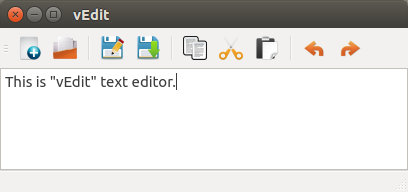
\includegraphics[scale=0.7]{images/vedit.png}
\caption{vEdit- The Text Editor}
\end{center}
\end{figure}

It has the following features:
\begin{itemize}
\item New File
\item Open File
\item Save File
\item Save as File
\item Copy
\item Paste
\item Cut
\item Undo
\item Redo
\end{itemize}

%Qt  is  designed  for  developing  applications  and  user  interfaces  once  and  deploying  them  across  several
%desktop and mobile operating systems. 
In this text editor we can make new text file and edit text. We can copy, cut and paste text easily. We can save and our text document in any location and open text document from any location. 

\subsection{Installation Guide}
To install vEdit, you need to clone it from github.
\begin{itemize}
\item Go to terminal and type\\\\
\textit{git clone http://www.github.com/mandeeps708/vEdit.git}
\item Now go to the directory vEdit by using: \\\\
\textit{cd vEdit}
\item Now running qmake command: \\\\
\textit{qmake vEdit.pro}
\item Now MakeFile will be generated. After that run make: \\\\
\textit{make}
\item An executable file will be generated. Execute it using: \\\\
\textit{./vEdit}
\end{itemize}
\section{Adding Features to LibreCAD v3}
During my 6 weeks training, I worked upon open source, learned a lot from it and in return contributed to it. LibreCAD v3 is written in C++ using Qt framework. It is a Qt application. With this project, I aimed at understanding C++ more clearly and deeply.\\
I added these features in LibreCAD v3's User Interface:
\begin{enumerate}
\item Open
\item Save 
\item Save As
\end{enumerate}
\begin{figure}[!ht]
\centering
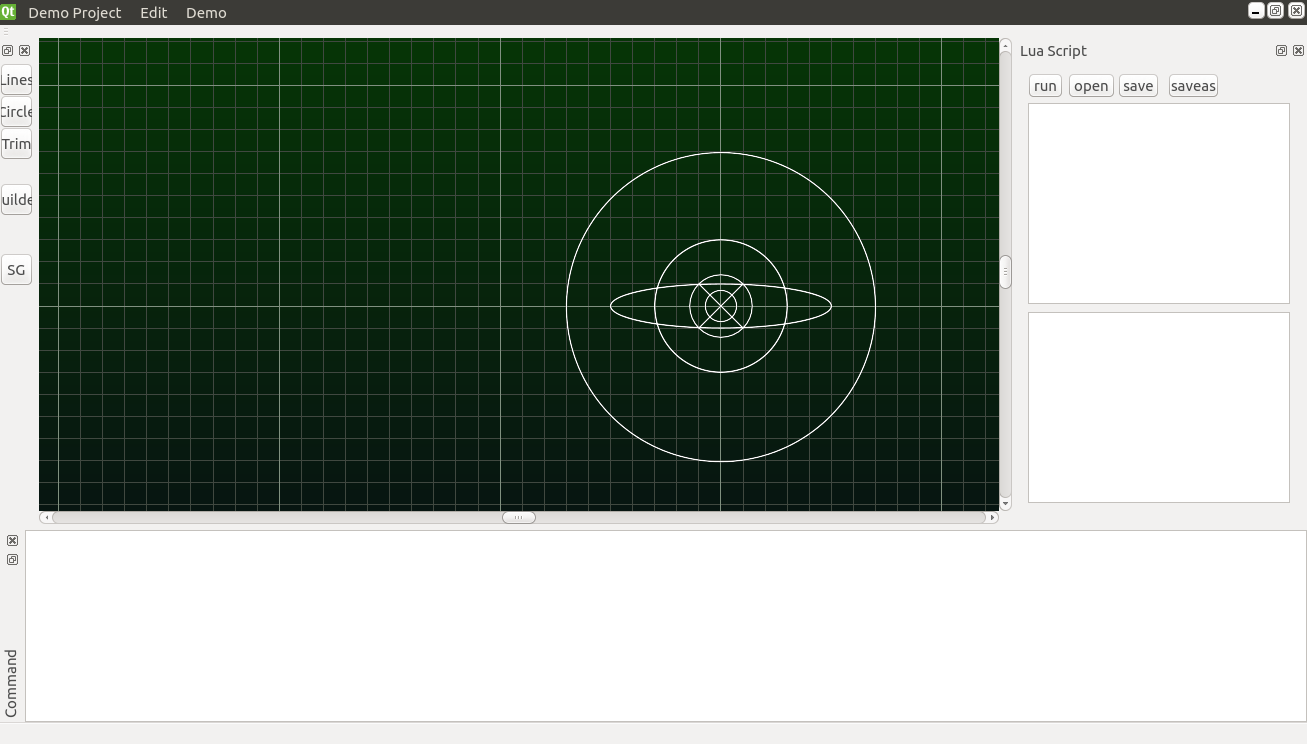
\includegraphics[scale=0.3]{images/ui.png}
\vspace{-1em}
\caption{Solid Fill: hatch.svg}
\hspace{-1.5em}
\end{figure}

\subsubsection{Open}
In this, I added Open feature to LibreCAD v3. This adds a button to the User Interface. When it is clicked, it prompts for a file to be opened. Then choose existing file and click "open". The file will be opened.\\
\begin{figure}[!ht]
\centering
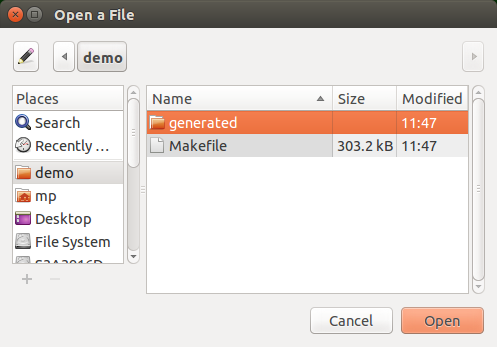
\includegraphics[scale=0.4]{images/open.png}
\vspace{-1em}
\caption{Open a File Prompt Box}
\hspace{-1.5em}
\end{figure}
\subsubsection{Save As}[!ht]
In this feature, when user clicks on "Save As" button, it prompts for a file location on which the file is to be saved.
\begin{figure}[!ht]
\centering
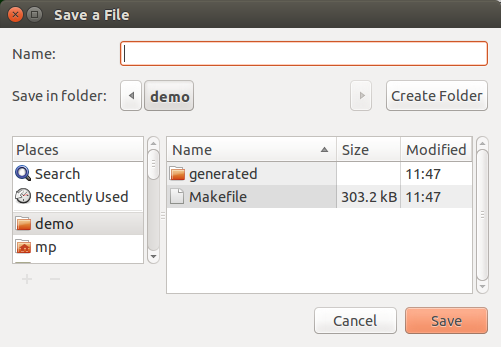
\includegraphics[scale=0.4]{images/save.png}
\vspace{-1em}
\caption{Save As Prompt Box}
\hspace{-1.5em}
\end{figure}
\subsubsection{Save}
In this feature, when user clicks on save button, it saves the script. It saves the changes to the existing file. 
 
\section{Design implementation using Lua scripting language}
After working with libreCAD 3, I experimented with it by making some designs usign Lua scripting language.
\noindent In this project, I made  several lua scripts and run it in LibreCAD to make various design. I made design of water tank and varoius logos and some other impressive 2D design in LibreCAD using LUA scripting language. 
In LibreCAD v3, there is a dockable window for creating lua scipts:
\begin{figure}[!ht]
\centering
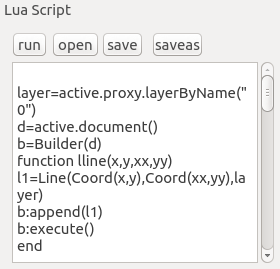
\includegraphics[scale=0.7]{images/lualogo/lua.png}                   
\vspace{-1em}
\caption{Lua Dockable window }
\hspace{-1.5em}
\end{figure}
\begin{figure}
\begin{center}
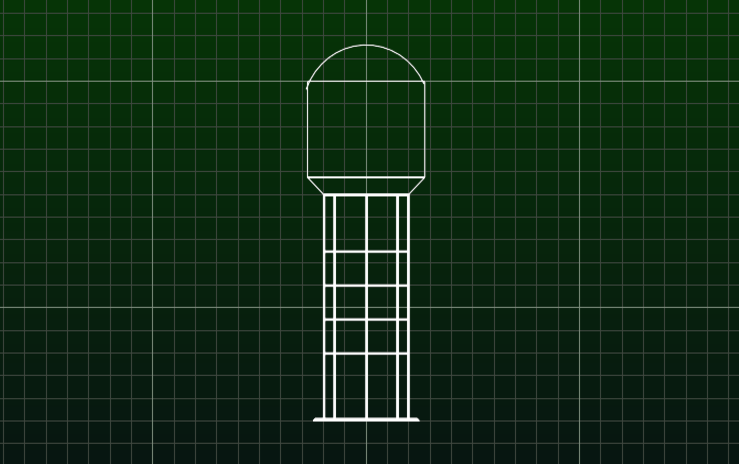
\includegraphics[scale=0.5]{images/lualogo/w2.png}
\caption{Water Tank Model}

\includegraphics[scale=0.5]{images/lualogo/batman.png} 
\caption{Batman Logo}
%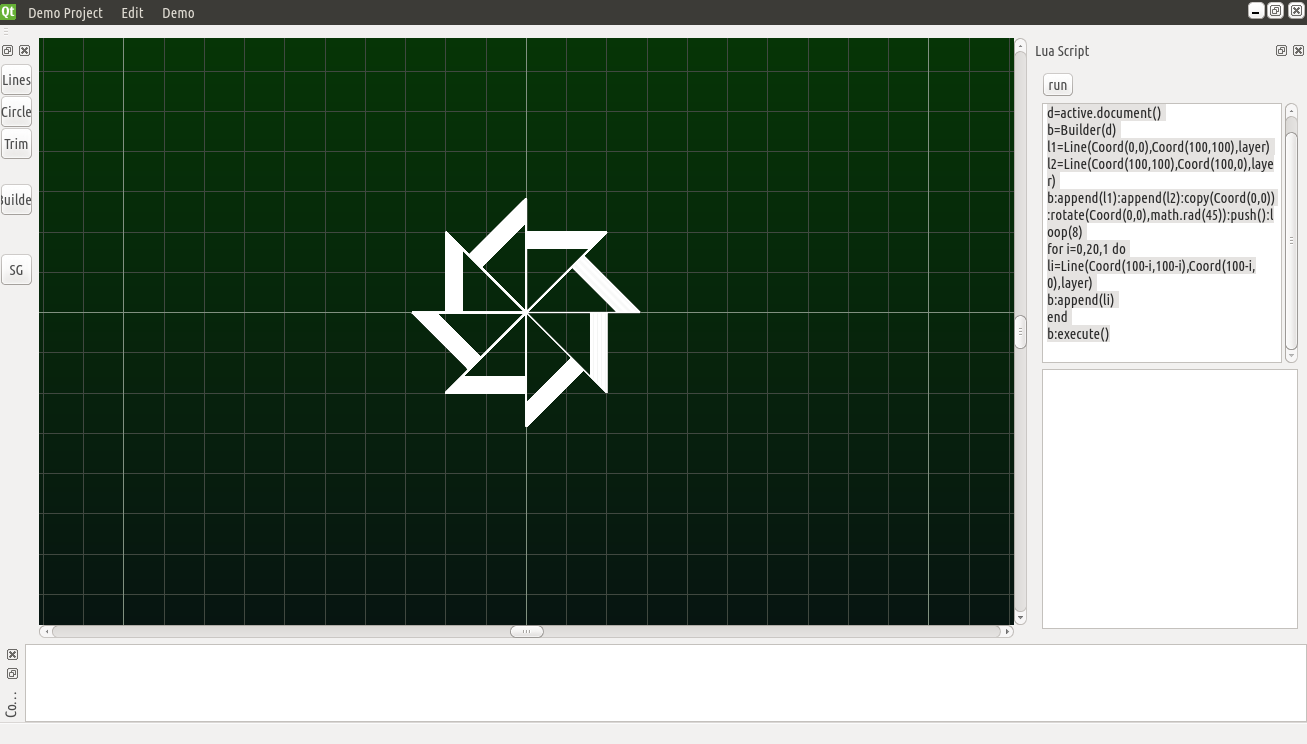
\includegraphics[scale=0.4]{images/lualogo/chakra1.png}
%\caption{Sharp Design 1}
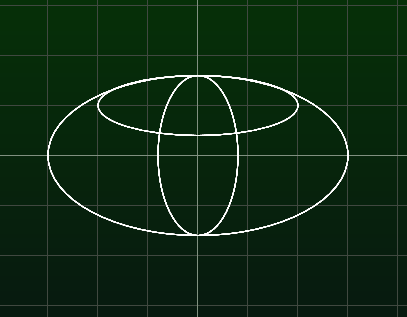
\includegraphics[scale=0.4]{images/lualogo/toyota.png}
\caption{Toyota Logo}
\end{center}
\end{figure}

\newpage
\section{Hatching}
This project also involves hatching implementation. To accomplish this, C++ and a graphics library named "Cairo" is used.
%\subsection{Introduction}
Basically, Hatching is a pattern of lines and dots that fills an enclosed area. Hatching can be used simply for color. The colors can represent materials or uses in drawings and renderings. There aren't any conventions for use of color in architecture. However, many other disciplines, such as urban planning and cartography, prescribe uses for colors in drawings and maps.
\noindent During the training, I also worked on Hatching. Basically, I have used C++ and a graphics library called Cairo. 
In this project, I've implemented two types of hatching:
\begin{enumerate}
\item Solid fill
\item Pattern fill
\end{enumerate}
\subsection{Solid fill}
\begin{itemize}
\item For Solid Fill, I made a C++ program named "solid.cpp" with help of Cairo graphics library. When it is compiled using:\\
\textit g++ solid.cpp -o output -lcairo
\item Then the executable will be created named "output". Execute it using:\\
\textit ./output
\item Then a file will be created named "hatch.svg" with the given color.
We can simply open it in terminal using command:\\
\textit eog hatch.svg
\begin{figure}[!ht]
\centering
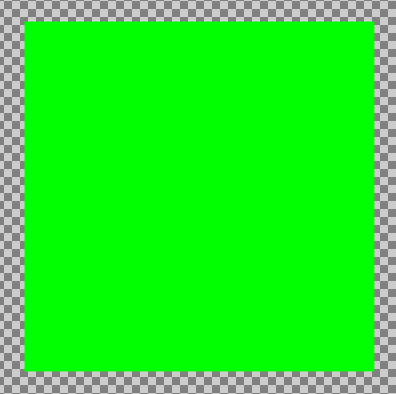
\includegraphics[scale=0.7]{images/hatching/solid.png}                   
\vspace{-1em}
\caption{Solid Fill: hatch.svg}
\hspace{-1.5em}
\end{figure}
\end{itemize}
\subsection{Pattern Fill}
\begin{itemize}
\item For Pattern Filling, I made another program named "pattern.cpp". When it is compiled using:\\
\textit{g++ pattern.cpp -o pexec -lcairo}
\item Then an executable file will be created named "pexec" in the current directory. Execute it using command:\\
\textit{./pexec}
\item Then a file will be created named "hello.png" which contains the hatched object.
Open this file using: \\
\textit{eog hello.png}
%\begin{figure}
%
\includegraphics[scale=0.7]{images/hatching/pattern.png}
%\caption{Pattern Fill: hello.png
%\end{figure}
\begin{figure}[!ht]
\centering

\includegraphics[scale=0.7]{images/hatching/pattern.png}                   
\vspace{-1em}
\caption{Pattern Fill: hello.png}
\hspace{-1.5em}
\end{figure}

\end{itemize}
\newpage
\chapter{Technologies Used}

\section{Introduction to Qt}

Qt Creator is a complete IDE for creating applications with Qt Quick and the Qt application framework.
Qt  is  designed  for  developing  applications  and  user  interfaces  once  and  deploying  them  across  several
desktop and mobile operating systems.
One  of  the  major  advantages  of  Qt  Creator  is  that  it  allows  a  team  of  developers  to  share  a  project
across  different  development  platforms  (Microsoft  Windows,  Mac  OS  X,  and  Linux)  with  a  common
tool  for  development and debugging. In addition, UI  designers can join the team by using Qt Quick tools
for creating fluid user interfaces in close cooperation with the developers.
The  main  goal  for  Qt  Creator  is  meeting  the  development  needs  of  Qt  Quick  developers  who  are
looking  for  simplicity, usability, productivity, extendibility and openness,  while aiming  to lower the barrier
of  entry  for  newcomers  to  Qt  Quick  and  Qt.  The  key  features  of  Qt  Creator  allow  UI  designers  and
developers to accomplish the following tasks:
\begin{itemize}
\item Get  started  with  Qt  Quick  application  development  quickly  and  easily  with  examples,  tutorials,
and project wizards.
\item Design  application  user  interface  with  the  integrated  editor,  Qt  Quick  Designer,  or  use graphics
software to design the user interface and use scripts to export the design to Qt Quick Designer.
\item Develop  applications   with  the   advanced  code  editor  that  provides  new  powerful  features  for
copleting code snippets, refactoring code, and viewing the element hierarchy of QML files.
\item Build  and  deploy  Qt  Quick  applications  that  target  multiple  desktop and mobile platforms, such
as Microsoft Windows, Mac OS X, Linux, Symbian, MeeGo, and Maemo.
\item Debug  JavaScript  functions  and  execute  JavaScript  expressions  in  the  current  context,   and
inspect QML at runtime to explore the object structure, debug animations, and inspect colors.
\item Profile  your  Qt  Quick  applications  with  the  QML  Profiler.  You can inspect binding evaluations,
signal  handling,  and  painting  operations  when  running  QML  code.  This  is  useful  for  identifying
potential bottlenecks, especially in the evaluation of bindings.
\item Deploy  applications  to  mobile  devices  and  create  application  installation  packages  for  Symbian
and Maemo devices that can be published in the Ovi Store and other channels.
\item Easily access information with the integrated context­sensitive Qt Help system.
\item It has differents modes such as Welcome, edit debug, design,analyze and help
\end{itemize}


\section{Working with Qt Creator}

Qt  Creator  meets  its  design  goals  of  simplicity,  ease­of­use,  and  productivity  by  relying  on the concept
of  modes.  These  adapt  the   user  interface  to  the  different  application  development  tasks  at  hand.  When
developers  start  Qt  Creator, it opens to  the Welcome mode, where they  can open tutorials and example
projects or start the project wizard to create their own projects.

\begin{figure}[h]
\begin{center}
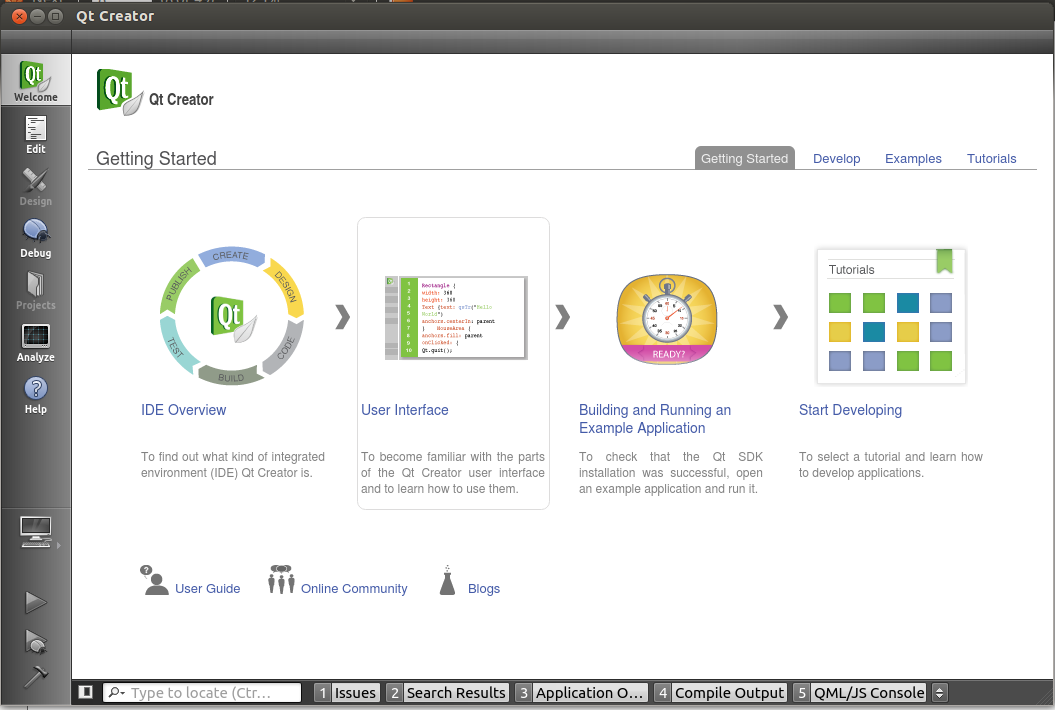
\includegraphics[scale=0.4]{images/Qt.png}
\caption{Welcome screen of Qt Creator}
\end{center}
\end{figure}

Each  mode  has  its  own  view  that  shows  only  the  information  required  for  performing  a  given  task,   and
provides  only  the  most  relevant  features  and  functions  related  to  it.  As  a  result,  the  majority  of  the  Qt
Creator window area is always dedicated to actual application development tasks.
Users  can  employ  the  mode  selector  to  switch  to  a  Qt  Creator  mode.  The  following  image  displays an
example application in Edit mode and Design mode.

\begin{figure}[h]
\begin{center}

\includegraphics[scale=0.8]{images/welcome.png}
\end{center}
\caption{Welcome mode in Qt}
\end{figure}
\begin{figure}[!h]
\begin{center}

\includegraphics[scale=0.8]{images/edit.png}
\caption{Edit mode in Qt}
\end{center}
\end{figure}

\newpage



\subsection{Creating Projects}

To  be  able  to  build  and  run  applications,  Qt  Creator  needs  the  same  information  as  a  compiler  would
need.  This  information  is  specified  in  the  project  build  and  run  settings.  Setting  up  a  new  project  in  Qt
Creator  is  aided  by  a  wizard  that  guides  the  user  step­by­step  through  the  project  creation  process. 
\begin{figure}[htb]
\begin{center}
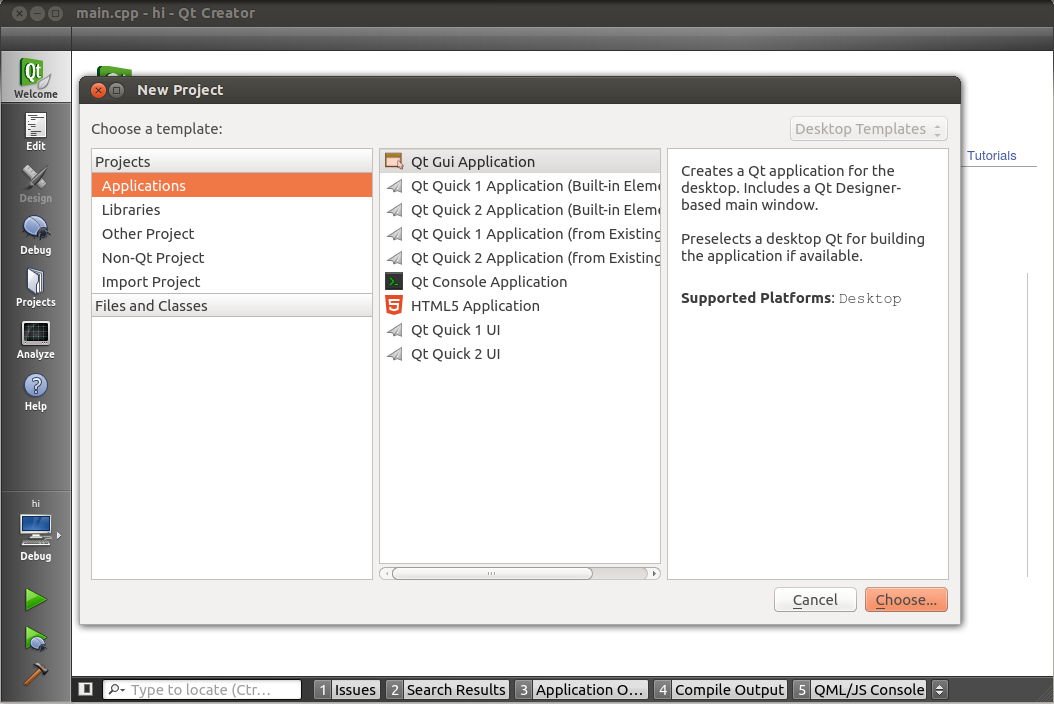
\includegraphics[scale=0.4]{images/new.png}
\caption{New file or project in Qt}
\end{center}
\end{figure}
In the  first  step,  the  user  selects  the  type of project from the categories. When  creating Qt Quick Projects,
the user can select either Qt Quick UI or Qt Quick Application.
A  Qt  Quick  UI  project  contains  a  single  QML  file  that  defines  the  main  view  of  the  application.  UI
designers  can  use  it  to  create  an  application  user  interface  and  review  it  in  the  QML  Viewer,  without
having  to  build  the  application.   UI  designers  do  not  need to have the development environment installed
on their computers to create and run this type of projects.
Developers  can  build  Qt  Quick  applications  and  deploy  them  on  mobile  target platforms. For example,
they  can  create  signed  Symbian  Installation  System  (SIS)  packages or Debian packages for this type of
project.  Developers  can  use  ready­made  Qt  Quick  Components  for  Symbian  and  MeeGo  Harmattan
that  allow  them  to  create  applications  with  a  native  look  and  feel  for  the  selected  mobile  platform.  The
components  are  delivered  as  part  of  Qt SDK. A Qt Quick UI project can be easily  converted into a Qt
Quick  application  by using the Qt Quick  application wizard to import the main QML file in the Qt Quick
UI project. The wizard prompts developers to enter the settings needed for a particular type of project.

\begin{figure}[h]
\begin{center}
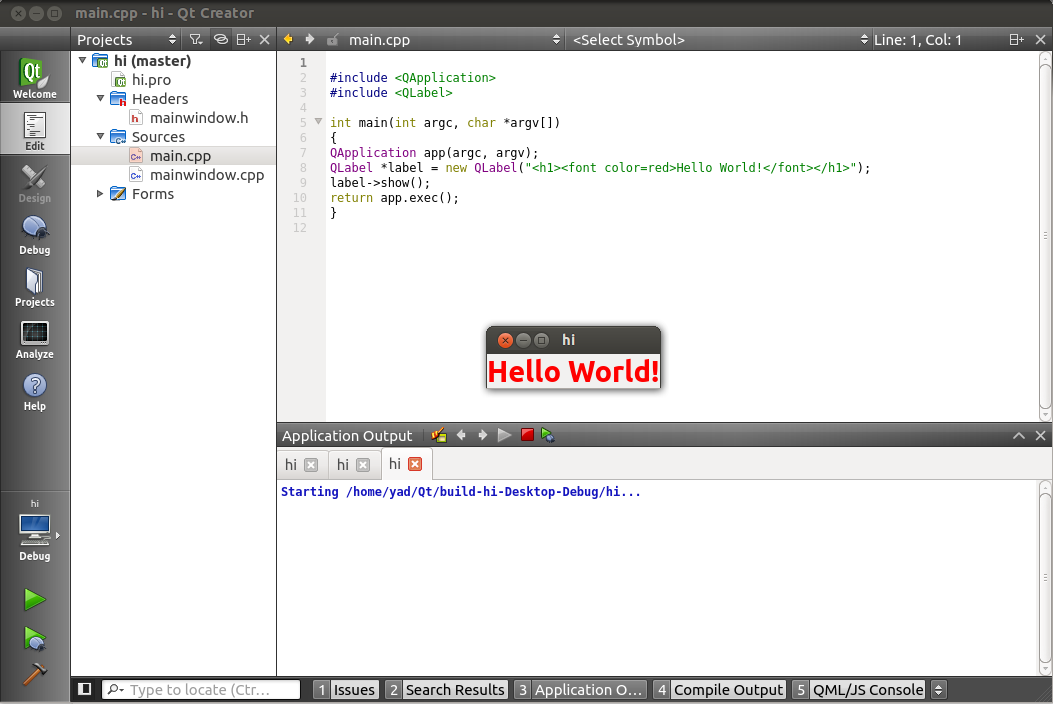
\includegraphics[scale=0.4]{images/hi.png}
\caption{Project to print hello word}
\end{center}
\end{figure}

When  the  steps  have  been  completed,  Qt  Creator  automatically  generates  the  project  with  required
headers,  source  files,  user  interface  descriptions  and  project  files,  as  defined  by  the  wizard.  Not  only
does  the  wizard  help  new  users  get  up  and  running  quickly,  it  also  enables  more  experienced  users  to
streamline  their  workflow  for  the  creation  of new projects. The convenient user interface makes it easier
to  ensure  that  a  project  begins  with  the  correct  configuration  and  dependencies.  Specifically,  the  Qt
Quick  application  wizard  allows  developers  to  create  projects  that  they  can  deploy  on  mobile  devices
with a click of the run button.
\\


\subsection{Using Qt Quick Toolbars}


When  users  edit  QML  code  in  the  code  editor,  they  specify  the  properties  of  QML   components.  For
some  properties,  such  as  colors   and  font  names,  this  is  not  a  trivial  task.  For  example,  few  people  can
visualize the color.
To  easily  edit these properties, users can employ the Qt Quick Toolbars. When a component is selected
in  the  code  and  a  toolbar  is  available,  a  light  bulb  icon  appears.  Users  select  the  icon  to  open  the
toolbar.
Qt  Quick  Toolbar  indicator  and  Qt  Quick  Toolbar  for  rectangles.  It  is  used  for  inserting  text,  images,
and  animation.  Qt  Quick  Toolbars  are  available  for  editing  the  properties  of  the  following  QML
elements:
● Rectangles
● Text
● Images
● Animation


\subsection{Deploying Applications to Mobile Devices}

Qt Creator deploy configurations handle the packaging of the application as an executable and copying it
to  a  location  developers  want  to  run  the  executable  at.  The  files  can  be  copied  to  a  location  in  the  file
system  of  the  development  PC  or  a  mobile  device.  To  deploy  files  on  mobile devices, developers must
either  connect  the  devices  to  the  development  PC  or  use  the  installation  packages  generated  by  Qt
Creator.  Qt  Quick  UI  projects  must  be  converted into Qt Quick applications for deployment on mobile devices.
Qt  Creator  allows developers to  create installation packages for Symbian, MeeGo, and Maemo devices
that are suitable for publishing on Ovi Store.


%----------------------------------------------------------------------------------------
\
\
\
%-------------------------------------------------------------------


\subsection{Getting Help}

From  time  to  time,  developers  may  need  further  information  about  a  certain  QML  element,  Qt  class,
function,  or  other  part  of  the  Qt  API.  All   the  Qt  documentation  and  examples are accessible via the Qt
Help plugin in Qt Creator.
To  view  the  documentation,   the  Help  mode  is  used,  where  most  of  the  window  is  devoted  to  the  help
text.  While working with source code in Edit mode, the user can access context sensitive help by moving
the  text  cursor  to  a  Qt  class  or   function  and  then  press  the  F1  key.  The  documentation  is  displayed
within a panel on the right side of the code editor, as shown in the following figure.

Qt  Designer  is  a  powerful cross­platform GUI layout and forms builder. It allows you to rapidly design
and  build  widgets  and  dialogs  using  on­screen  forms  using  the  same  widgets  that  will  be  used  in  your
application.  Forms  created  with  Qt  Designer  are fully­functional, and they can be previewed so that you
can ensure that they will look and feel exactly as you intended.\\


%----------------------------------------------------------------------------------------

%-------------------------------------------------------------------

\begin{small}
\subsection{\large Features and Benefits}
\end{small}
\begin{itemize}
\item Design user interfaces quickly with drag and drop functionality
\item Customize widgets or choose from library of standard widgets
\item Instantly preview forms in native look and feel
\item Generate C++ or Java code from your interface prototypes
\item Use Qt Designer with Visual Studio or Eclipse IDEs
\item Build fully­functional user interfaces with Qt’s signals and slots
\end{itemize}
\begin{figure}[htb]
\begin{center}
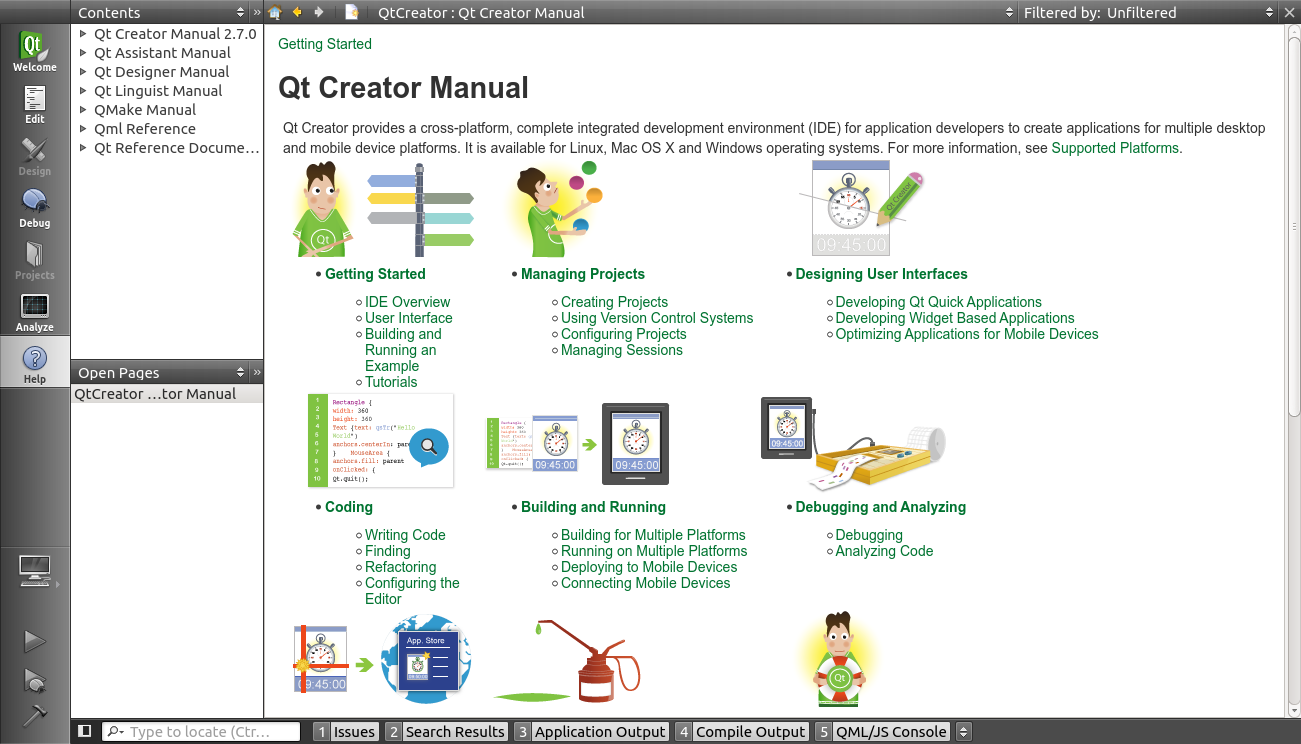
\includegraphics[scale=0.4]{images/Qtman.png}
\caption{ Displaying context sensitive Qt Help information}
\end{center}
\end{figure}
\newpage
\section{Introduction to \LaTeX}

\LaTeX, I had never heard about this term before doing this project,
but when I came to know about its features, found it excellent. 
\LaTeX{} (pronounced /ˈleɪtɛk/, /ˈleɪtɛx/, /ˈlɑːtɛx/, or /ˈlɑːtɛk/) is a 
document markup language and document preparation system for the \TeX{} 
typesetting  program. Within the typesetting system, its name is styled 
as \LaTeX.

\image{0.9}{images/donald.png}{Donald Knuth, Inventor Of \TeX{} 
typesetting system}

Within the typesetting system, its name is styled as \LaTeX. The term 
\LaTeX{} refers only to the language in which documents are written, 
not to the editor used to write those documents. In order to create a 
document in \LaTeX, a .tex file must be created using some form of text 
editor. While most text editors can be used to create a \LaTeX{} document, 
a number of editors have been created specifically for working with \LaTeX.

\LaTeX{} is most widely used by mathematicians, scientists, 
engineers, philosophers, linguists, economists and other scholars in 
academia. As a primary or intermediate format, e.g., translating DocBook 
and other XML-based formats to PDF, \LaTeX{} is used because of the 
high quality of typesetting achievable by \TeX. The typesetting system 
offers programmable desktop publishing features and extensive facilities 
for automating most aspects of typesetting and desktop publishing, 
including numbering and cross-referencing, tables and figures, 
page layout and bibliographies.

\LaTeX{} is intended to provide a high-level language that
accesses the power of \TeX. \LaTeX{} essentially comprises a
collection of \TeX{} macros and a program to process \LaTeX documents. 
Because the \TeX{} formatting commands are very low-level, it is usually 
much simpler for end-users to use \LaTeX{}.


\subsection{Typesetting}
\LaTeX{} is based on the idea that authors should be able to focus on 
the content of what they are writing without being distracted by its 
visual presentation. In preparing a \LaTeX{} document, the author 
specifies the logical structure using familiar concepts such as 
chapter, section, table, figure, etc., and lets the \LaTeX{} system 
worry about the presentation of these structures. It therefore 
encourages the separation of layout from content while still allowing 
manual typesetting adjustments where needed. 

\begin{verbatim}
\documentclass[12pt]{article}
\usepackage{amsmath}
\title{\LaTeX}
\date{}
\begin{document}
  \maketitle 
  \LaTeX{} is a document preparation system 
  for the \TeX{} typesetting program.
   \par 
   $E=mc^2$
\end{document}
\end{verbatim}
\image{0.3}{images/latexoutput.png}{\LaTeX{} output of above program.}

\subsection{Installing \LaTeX{} on System}
Installation of \LaTeX{} on personal system is quite easy. As i have used \LaTeX{} on Ubuntu 13.04 so i am discussing the installation steps for Ubuntu 13.04 here:
\begin{itemize}
\item Go to terminal and type\\\\
\textit{sudo apt-get install texlive-full}
\item Your Latex will be installed on your system and you can check for manual page by typing.\\\\
\textit{man latex}\\
in terminal which gives manual for latex command.\\
\item To do very next step now one should stick this to mind that the document which one is going to produce is written in any type of editor whether it may be your most common usable editor Gedit or you can use vim by installing first vim into your system using command.\\\\
\textit{sudo apt-get install vim}\\
\item After you have written your document it is to be embedded with some set of commands that Latex uses so as to give a structure to your document. Note that whenever you wish your document to be looked into some other style just change these set of commands.\\\\
\item When you have done all these things save your piece of code with .tex format say test.tex. Go to terminal and type\\\\
\textit{latex path of the file test.tex Or pdflatex path of the file test.tex\\ eg: pdflatex test.tex}\\
for producing pdf file simultaneously.\\
After compiling it type command\\\\
\textit{evince filename.pdf\\ eg: evince test.pdf}\\
To see output pdf file. 
\end{itemize}

\subsection{Graphical Editors for \LaTeX{}}
\LaTeX{} is not restricted to command line only there are so many graphical based editors available to be used. These GUi based editors provide an easy interface to user so as to do typesetting in an efficient manner. Some of them are listed below:
\begin{itemize}
\item {Texmaker}
\begin{figure}[ht]
\centering
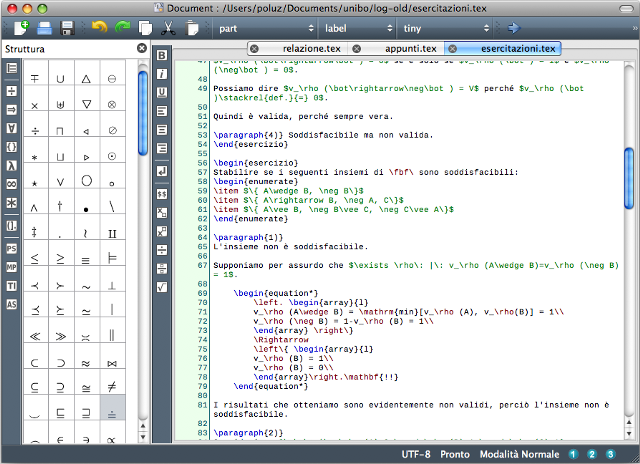
\includegraphics[scale=0.4]{images/texmaker.png}
\caption{Texmaker, A Graphical \LaTeX{} Editor}
\end{figure}
\item LEd
\begin{figure}[ht]
\centering
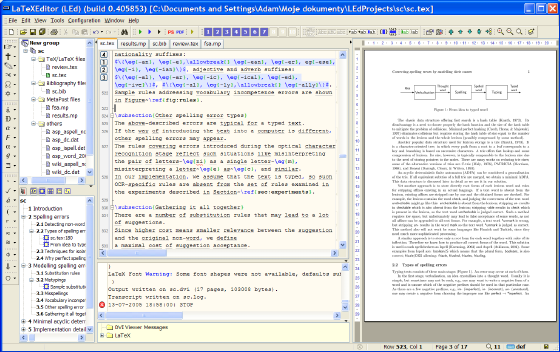
\includegraphics[scale=0.5]{images/led.png}
\caption{LEd, A Graphical \LaTeX{} Editor}
\end{figure}
\end{itemize}
And many more but the preferred method to produce \LaTeX{} document is through console mode only.


\subsection{Pdfscreen \LaTeX{}}
There are some packages that can help to have unified document using \LaTeX{}. Example of such a package is pdfscreen that let the user view it’s document in two forms-print and screen. Print for hard copy and screen for viewing your document on screen. Download this package from www.ctan.org/tex-archive/macros/latex/contrib/pdfscreen/.\\
Then install it using above mention method.\\
To test it the test code is given below:-\\
Just changing print to screen gives an entirely different view. But for working of pdfscreen another package required are comment and fancybox.\\\\
The fancybox package provides several different styles of boxes for framing and rotating content in your document. Fancybox provides commands that produce square-cornered boxes with single or double lines, boxes with shadows, and round-cornered boxes with normal or bold lines. You can box mathematics, floats, center, flushleft, and flushright, lists, and pages.\\\\
Whereas comments package selectively include/excludes portions of text. The comment package allows you to declare areas of a document to be included or excluded. One need to make these declarations in the preamble of your file. The package uses a method for exclusion that is pretty robust, and can cope with ill-formed bunches of text.\\\\
So these extra packages needed to be installed on system for the proper working of pdfscreen package.
\subsection{Web based graphic generation using \LaTeX{}}
\LaTeX{} is also useful when there is need of generating the graphics from browser. For
example to draw a circle by just entering its radius in html input box. So this kind
A
of project can be conveniently handled using \LaTeX{}. Basic idea behind this generation
process is that when user clicks on submit button after entering radius a script will run
that enter the radius in already made .tex file and recompiles it on server and makes its
pdf and postscript file. After that user can view those files by clicking on link provided
to view the files. See some screen shots of such a graphic generation project made by
Dr. H.S. Rai:\\
So here in the above input page which is also the index page user can enter input
for length of rectangle, breadth of rectangle and for radius of circle after that user can submit the values. After the values get submitted a script get runs by php code at server
side. This script first enters the dimensions of rectangle and circle that were selected by
user in to an already existing .tex file and replace with the older dimensions there. After
that script recompiles the the tex file and make it available for user.\\
In above figure it gets clear that .tex file has been compiled and pdf and postscript files
are available to user and user can download the graphics so produced. Hence graphics
can be generated in \LaTeX{} through web interface.
\begin{figure}[ht]
\centering
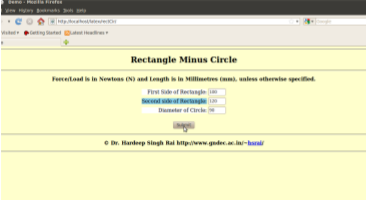
\includegraphics[scale=0.5]{images/webgraphic.png}
\caption{Web based graphic generation using \LaTeX{}(input page)}
\end{figure}

\section{Introduction to Lua scripting language}
\begin{figure}[!ht]
\centering

\includegraphics[width=0.3\textwidth]{images/lua.png} 
\vspace{-0.5em}
\caption{Lua Logo}
\hspace{-1.5em}
\end{figure}
\leavevmode\\
Lua is a powerful and fast programming language that is easy to learn and use and to embed into your application. Lua is designed to be a lightweight embeddable scripting language and is used for all sorts of applications from games to web applications and image processing.\\\\
Lua combines simple procedural syntax with powerful data description constructs based on associative arrays and extensible semantics. Lua is dynamically typed, runs by interpreting bytecode for a register-based virtual machine, and has automatic memory management with incremental garbage collection, making it ideal for configuration, scripting, and rapid prototyping.\\\\

\subsection{Installation of Lua}
Lua is implemented in pure ANSI C and compiles unmodified in all platforms that have an ANSI C compiler. Lua also compiles cleanly as C++. The current version is lua-5.2.3. Just download the source from the lua.org/download and then follow the steps for building it\\\\
\emph
{curl -R -O http://www.lua.org/ftp/lua-5.2.3.tar.gz\\
tar zxf lua-5.2.3.tar.gz\\
cd lua-5.2.3\\
make
}

\leavevmode\\\\

\subsection{Why choose Lua?}
\begin{itemize}
\item \textbf{Lua is a proven, robust language}\\
Lua has been used in many industrial applications (e.g., Adobe's Photoshop Lightroom), with an emphasis on embedded systems (e.g., the Ginga middleware for digital TV in Brazil) and games (e.g., World of Warcraft and Angry Birds). Lua is currently the leading scripting language in games. Lua has a solid reference manual and there are several books about it. Several versions of Lua have been released and used in real applications since its creation in 1993. Lua featured in HOPL III, the Third ACM SIGPLAN History of Programming Languages Conference, in June 2007. 
\item \textbf{Lua is fast}\\
Lua has a deserved reputation for performance. To claim to be "as fast as Lua" is an aspiration of other scripting languages. Several benchmarks show Lua as the fastest language in the realm of interpreted scripting languages. Lua is fast not only in fine-tuned benchmark programs, but in real life too. Substantial fractions of large applications have been written in Lua. 
\item \textbf{Lua is portable}\\
Lua is distributed in a small package and builds out-of-the-box in all platforms that have a standard C compiler. Lua runs on all flavors of Unix and Windows, on mobile devices (running Android, iOS, BREW, Symbian, Windows Phone), on embedded microprocessors (such as ARM and Rabbit, for applications like Lego MindStorms), on IBM mainframes, etc. 
\item \textbf{Lua is embeddable}\\
 Lua is a fast language engine with small footprint that you can embed easily into your application. Lua has a simple and well documented API that allows strong integration with code written in other languages. It is easy to extend Lua with libraries written in other languages. It is also easy to extend programs written in other languages with Lua. Lua has been used to extend programs written not only in C and C++, but also in Java, C\#, Smalltalk, Fortran, Ada, Erlang, and even in other scripting languages, such as Perl and Ruby. 
\item \textbf{Lua is powerful (but simple)}\\
 A fundamental concept in the design of Lua is to provide meta-mechanisms for implementing features, instead of providing a host of features directly in the language. For example, although Lua is not a pure object-oriented language, it does provide meta-mechanisms for implementing classes and inheritance. Lua's meta-mechanisms bring an economy of concepts and keep the language small, while allowing the semantics to be extended in unconventional ways.
\item \textbf{Lua is small}\\
 Adding Lua to an application does not bloat it. The tarball for Lua 5.2.3, which contains source code and documentation, takes 246K compressed and 960K uncompressed. The source contains around 20000 lines of C. Under Linux, the Lua interpreter built with all standard Lua libraries takes 182K and the Lua library takes 244K. 
\item \textbf{Lua is free}\\
 Lua is free open-source software, distributed under a very liberal license (the well-known MIT license). It may be used for any purpose, including commercial purposes, at absolutely no cost. Just download it and use it. 
\end{itemize}

\newpage
\section{Introduction to Cairo Graphics Library}
Cairo is a library for creating 2D vector graphics. It is written in the C programming language. Bindings for other computer languages exist. Python, Perl, C++, C\#, Java. Cairo is a multiplatform library, it works on Linux, BSDs, and Mac OS.\\

\begin{center}
%
\includegraphics[scale=0.8]{images/cairo.png}
\image{0.9}{images/cairo.png}{Cairo Logo}
%\caption{Cairo Logo}
\end{center}

Cairo supports various backends:
\begin{itemize}
\item X Window System
\item Win32 GDI
\item Mac OS X Quartz
\item PNG
\item PDF
\item PostScript
\item SVG
\end{itemize}

\noindent This means that we can use the library to draw on windows on Linux/BSDs, Windows, Mac OS and we can use the library to create PNG images, PDF files, PostScript files, and SVG files.

\section{Introduction to Github}
\begin{figure}[!ht]
\centering

\includegraphics[width=0.3\textwidth]{images/github}                   
\vspace{-1em}
\caption{Github Logo}
\hspace{-1.5em}
\end{figure}
\leavevmode\\
GitHub is a Git repository web-based hosting service which offers all of the functionality of Git as well as adding many of its own features. Unlike Git which is strictly a command-line tool, Github provides a web-based graphical interface and desktop as well as mobile integration. It also provides access control and several collaboration features such as wikis, task management, and bug tracking and feature requests for every project.\\

GitHub offers both paid plans for private repto handle everything from small to very large projects with speed and efficiency. ositories, and free accounts, which are usually used to host open source software projects. As of 2014, Github reports having over 3.4 million users, making it the largest code host in the world.\\

GitHub has become such a staple amongst the open-source development community that many developers have begun considering it a replacement for a conventional resume and some employers require applications to provide a link to and have an active contributing GitHub account in order to qualify for a job.\\\\

\section{What is Git?}
\begin{figure}[!ht]
\centering

\includegraphics[width=0.3\textwidth]{images/git}                   
\vspace{-1em}
\caption{Git Logo}
\hspace{-1.5em}
\end{figure}
Git is a distributed revision control and source code management (SCM) system with an emphasis on speed, data integrity, and support for distributed, non-linear workflows. Git was initially designed and developed by Linus Torvalds for Linux kernel development in 2005, and has since become the most widely adopted version control system for software development.\\

As with most other distributed revision control systems, and unlike most client–server systems, every Git working directory is a full-fledged repository with complete history and full version-tracking capabilities, independent of network access or a central server. Like the Linux kernel, Git is free and open source software distributed under the terms of the GNU General Public License version 2 to handle everything from small to very large projects with speed and efficiency.\\

Git is easy to learn and has a tiny footprint with lightning fast performance. It outclasses SCM tools like Subversion, CVS, Perforce, and ClearCase with features like cheap local branching, convenient staging areas, and multiple workflows.\\\\

\subsection{Installation of Git}

Installation of git is a very easy process.
The current git version is: 2.0.4.
Type the commands in the terminal:\\\\
\emph{
\$ sudo apt-get update\\\\
\$ sudo apt-get install git\\\\}
This will install the git on your pc or laptop.

\subsection{Various Git Commands}

Git is the open source distributed version control system that facilitates GitHub activities on your laptop or desktop. The commonly used Git command line instructions are:-\\



\subsection*{Create Repositories}
\addcontentsline{toc}{subsection}{Create Repositories}
Start a new repository or obtain from an exiting URL

\begin{description}

\item [\$ git init [ project-name]]\\
Creates a new local repository with the specified name
\item [\$ git clone [url]]\\
Downloads a project and its entire version history

\end{description}
\leavevmode \\


\subsection*{Make Changes}
\addcontentsline{toc}{subsection}{Make Changes}
Review edits and craft a commit transaction

\begin{description}

\item [\$ git status] \leavevmode \\
Lists all new or modified files to be committed

\item [\$ git diff] \leavevmode \\
Shows file differences not yet staged

\item [\$ git add [file]]\\
Snapshots the file in preparation for versioning

\item [\$ git reset [file]]\\
Unstages the file, but preserve its contents

\item [\$ git commit -m "[descriptive message]"]\\
Records file snapshots permanently in version history

\end{description}
\leavevmode \\


\subsection*{Group Changes}
\addcontentsline{toc}{subsection}{Group Changes}
Name a series of commits and combine completed efforts

\begin{description}

\item [\$ git branch] \leavevmode \\
Lists all local branches in the current repository

\item [\$ git branch [branch-name]]\\
Creates a new branch

\item [\$ git checkout [branch-name]]\\
Switches to the specified branch and updates the working directory

\item [\$ git merge [branch]]\\
Combines the specified branch’s history into the current branch

\item [\$ git branch -d [branch-name]]\\
Deletes the specified branch

\end{description}
\leavevmode \\


\subsection*{Save Fragments}
\addcontentsline{toc}{subsection}{Save Fragments}
Shelve and restore incomplete changes

\begin{description}

\item [\$ git stash] \leavevmode \\
Temporarily stores all modified tracked files

\item [\$ git stash pop] \leavevmode \\
Restores the most recently stashed files

\item [\$ git stash list] \leavevmode \\
Lists all stashed changesets

\item [\$ git stash drop] \leavevmode \\
Discards the most recently stashed changeset

\end{description}
\leavevmode \\


\subsection*{Synchronize Changes}
\addcontentsline{toc}{subsection}{Synchronize Changes}
Register a repository bookmark and exchange version history

\begin{description}

\item [\$ git fetch [bookmark]]\\
Downloads all history from the repository bookmark

\item [\$ git merge [bookmark]/[branch]]\\
Combines bookmark’s branch into current local branch

\item [\$ git push [alias][branch]]\\
Uploads all local branch commits to GitHub

\item [\$ git pull] \leavevmode \\
Downloads bookmark history and incorporates changes

\end{description}

%Github\\
%IRC\\
%\LaTeX\\
%Lua\\

%\input{input/techno-used.tex}
%\chapter{Design}
%\section{System Design} : Systems design is the process or art of defining 
the architecture, components, modules, interfaces, and data for a 
system to satisfy specified requirements. One could see it as the 
application of systems theory to product development. There is some 
overlap with the disciplines of systems analysis, systems architecture 
and systems engineering.
\begin{itemize}
\item  External design: External design consists of conceiving, 
planning out and specifying the externally observable characteristics 
of the software product. These characteristics include user displays 
or user interface forms and the report formats, external data sources 
and the functional characteristics, performance requirements etc. 
External design begins during the analysis phase
and continues into the design phase.
\item  Logical design: The logical design of a system pertains to an 
abstract representation of the data flows, inputs and outputs of the 
system. This is often conducted via modeling, which involves a 
simplistic (and sometimes graphical) representation of an actual 
system. In the context of systems design, modeling can undertake the 
following forms, including:
\begin{itemize}
\item Data flow diagrams
\item Entity Relationship Diagrams
\end{itemize}
\item  Physical design: The physical design relates to the actual 
input and output processes of the system. This is laid down in terms 
of how data is input into a system, how it is verified/authenticated, 
how it is processed, and how it is displayed as output.
\end{itemize}
\newpage
\section{Design Notations}
{\bf Data Flow diagrams}:
\image{0.6}{images/sss1.png}{DFD Notation}\\
\newpage
{\bf Flow Charts}:
\image{0.5}{images/sss2.png}{Flow Chart Notations}\\
%Entity Relationship Diagrams:
%\image{0.6}{images/sss3.png}{ER Diagram Notation}\\
{\centering \bf Detailed Design}
We basically describe the functionality of the system internally. 
The internal design describes how data is flowing from database to the 
user and how they both are internally connected. For this reason we 
can show the design of the system in detailed manner by many ways: \\\\
{\bf Flowchart } A flowchart is a type of diagram that represents an
algorithm or process, showing the steps as boxes of various kinds, and
their order by connecting them with arrows. This diagrammatic
representation can give a step-by-step solution to a given problem.
Process operations are represented in these boxes, and arrows
connecting them represent flow of control. Data flows are not
typically represented in a flowchart, in contrast with data flow
diagrams; rather, they are implied by the sequencing of operations.
Flowcharts are used in analyzing, designing, documenting or managing a
process or program in various fields
\newpage
\section{Database Design}
\image{0.4}{images/design.png}{Database Design}


%\chapter{Implementation}
%\input{input/implement.tex}
\chapter{Project Legacy}
\section{Technical and Managerial Lesson Learnt}
I learned a lot by doing this project . During this period I got to learn a vast 
number of technologies. These are listed below :
\begin{itemize}
\item {\bf{Operating system}}: Ubuntu
\item {\bf{Languages used}}: C++, Lua
\item {\bf{Framework}}: Qt 
\item {\bf{Typesetting}}: LaTex
\item {\bf{Other Learnings}}: Internet Relay Chat(IRC)

\end{itemize}

% Edit this file%
So during this project I learned all the above things. Above all I got to know 
how Softwares are developed from the scratch. Planning, designing, developing code, 
working in a team, testing etc. These are all very precious things I got to learn 
during this period.  

\subsection{Ubuntu: An open source OS}
During my training, I also got familiar with a great and open source Operating System, Ubuntu. Firstly, it was quite difficult for a regular MS Windows user to port to Ubuntu. I did all of my project work using this vast operating system. 
Ubuntu (/uːˈbuːntuː/ oo-BOON-too) is a Debian-based Linux operating system, with Unity as its default desktop environment. It is based on free software and named after the Southern African philosophy of ubuntu (literally, "human-ness"), which often is translated as "humanity towards others" or "the belief in a universal bond of sharing that connects all humanity".\\
Ubuntu's goal is to be secure "out-of-the box". By default user's programs run with low privileges and cannot corrupt the operating system or other user's files. For increased security, the sudo tool is used to assign temporary privileges for performing administrative tasks, which allows the root account to remain locked and helps prevent inexperienced users from inadvertently making catastrophic system changes or opening security holes.\\

\subsection{Internet Relay Chat}
Internet Relay Chat (IRC) is an application layer protocol that facilitates transfer of messages in the form of text. The chat process works on a client/server model of networking. IRC clients are computer programs that a user can install on their system. These clients are able to communicate with chat servers to transfer messages to other clients. It is mainly designed for group communication in discussion forums, called channels, but also allows one-to-one communication via private message as well as chat and data transfer, including file sharing.
Client software is available for every major operating system that supports Internet access.IRC is an open protocol that uses TCP and, optionally, TLS. An IRC server can connect to other IRC servers to expand the IRC network. Users access IRC networks by connecting a client to a server. There are many client implementations, such as mIRC, HexChat and irssi, and server implementations, e.g. the original IRCd. Most IRC servers do not require users to register an account but a user will have to set a nickname before being connected.\\

IRC has a line-based structure with the client sending single-line messages to the server,receiving replies to those messages and receiving copies of some messages sent by other clients. In most clients, users can enter commands by prefixing them with a '/'. Depending on the command, these may either be handled entirely by the client, or  passed directly to the server, possibly with some modification.\\

The basic means of communicating to a group of users in an established IRC session is through a channel. Channels on a network can be displayed using the IRC command LIST, which lists all currently available channels that do not have the modes +s or +p set, on that particular network.
Users can join a channel using the JOIN command, in most clients available as /join \#channelname. Messages sent to the joined channels are then relayed to all other users.\\
%\subsection{Shell Scripting}
%Because all my project
\section{Future Scope}
The  future  of  GUI  programming  in  my  opinion is Qt programming,  which involves the efficiency and low
levelness  of  C++  as  it’s  a  C++  framework  but  also  has  all  the  qualities  that  a  modern  programming
language  has.  It  gives  you  a  way  to  easily  develop  applications  and  GUIs  which  using  C++  was earlier
not  possible.  Open  source  is  always  growing  field  I  have  a  vision  that  LibreCAD  will  someday  be  as
famous  as  other  CAD  programs   such  as  Autocad.  This  is  the  dawn of Open Source Softwares and we
still  have  to  grow  a  lot.  I  have  added some new  features and in  LibreCAD, the LibreCAD is going to improve day by day. LibreCAD is completely scalable so
I  can  also add as many features as I want. Future  scope  is  bright  as  I  believe  that  this  is  just  the
beginning and there is allot more to learn and implement.

\begin{thebibliography}{9}
\bibitem{} LibreCAD 3, http://github.com/gaganjyot/LibreCAD\_3
\bibitem{} My Blog,
http://gurpindersingh751.wordpress.com
\bibitem{} My Github Profile,
http://github.com/gurpinder1001
\end{thebibliography}

\end{document}

